\section{Backpropagation and emission synthesis}\label{sec:tool:synthesis}

\subsection{Introduction}
The previous section treated the propagation model of the tool. In order to
simulate the audible sound of aircraft an emission signal is needed.
This section describes a method to create an emission signal from features derived from
recordings. An auralisation or pseudo-recording at a receiver position can then
be created by propagating the signal using the propagation model. Figure
\ref{fig:tool:backpropagation:introduction:block-diagram} shows a block diagram
of the steps that are treated in this section.

\begin{figure}[H]
  \centering
\begin{tikzpicture}[auto, node distance=1cm,>=latex']
\tikzset{
block/.style    = {draw, shape=rectangle, fill=white, minimum height=4em, minimum width=5em, text width=5em, align=center},
}
    % Main nodes
    \node [block]                       (recording)     {Recording};
    \node [block, right=of recording]   (backprop)      {Back-\\propagation};
    \node [block, right=of backprop]    (feature)       {Feature\\extraction};
    \node [block, right=of feature]     (emission)      {Emission\\synthesis};
%     \node [block, right=of emission]    (auralisation)  {Auralisation};

    % Main edges
    \draw [->]  (recording)     --  (backprop);
    \draw [->]  (backprop)      --  (feature);
    \draw [->]  (feature)       --  (emission);
%     \draw [->]  (emission)      --  (immission);

\end{tikzpicture}
  \caption{Block diagram of the backpropagation, synthesis and auralisation method.}
  \label{fig:tool:backpropagation:introduction:block-diagram}
\end{figure}

% An automated procedure was developed to a) backpropagate from source to receiver
% in time-domain and b) analyze the resulting signal to extract features that could be
% used in the development of an emission model or to directly resynthesise the
% emission.

% \subsection{Measurement data}

For the emission synthesis a signal is generated that is based on measurements
that were made for the sonAIR project as described in section
\ref{sec:introduction:sonair}. Figure \ref{fig:figure_trajectory} shows an
overview of the airport, the trajectory and the receiver of the events
considered. Aircraft took off and their height steadily increased from 30 to 260
meters.

% For the data presented measurements from only a single microphone
% were used, situated at a height of 4 meters.


% For the development of the sonAIR model \cite{Zellmann2016} sound recordings
% were made for a large amount of events nearby Z\"{u}rich Airport
% \cite{Zellmann2013}. Along with the sound recordings the position of the
% aircraft was registered and for a subset of the events more detailed information
% was obtained as well, like e.g. thrust settings. Recordings were made at
% multiple positions simultaneously, allowing to determine the directivity of the
% noise components.

\begin{figure}[H]
  \centering
  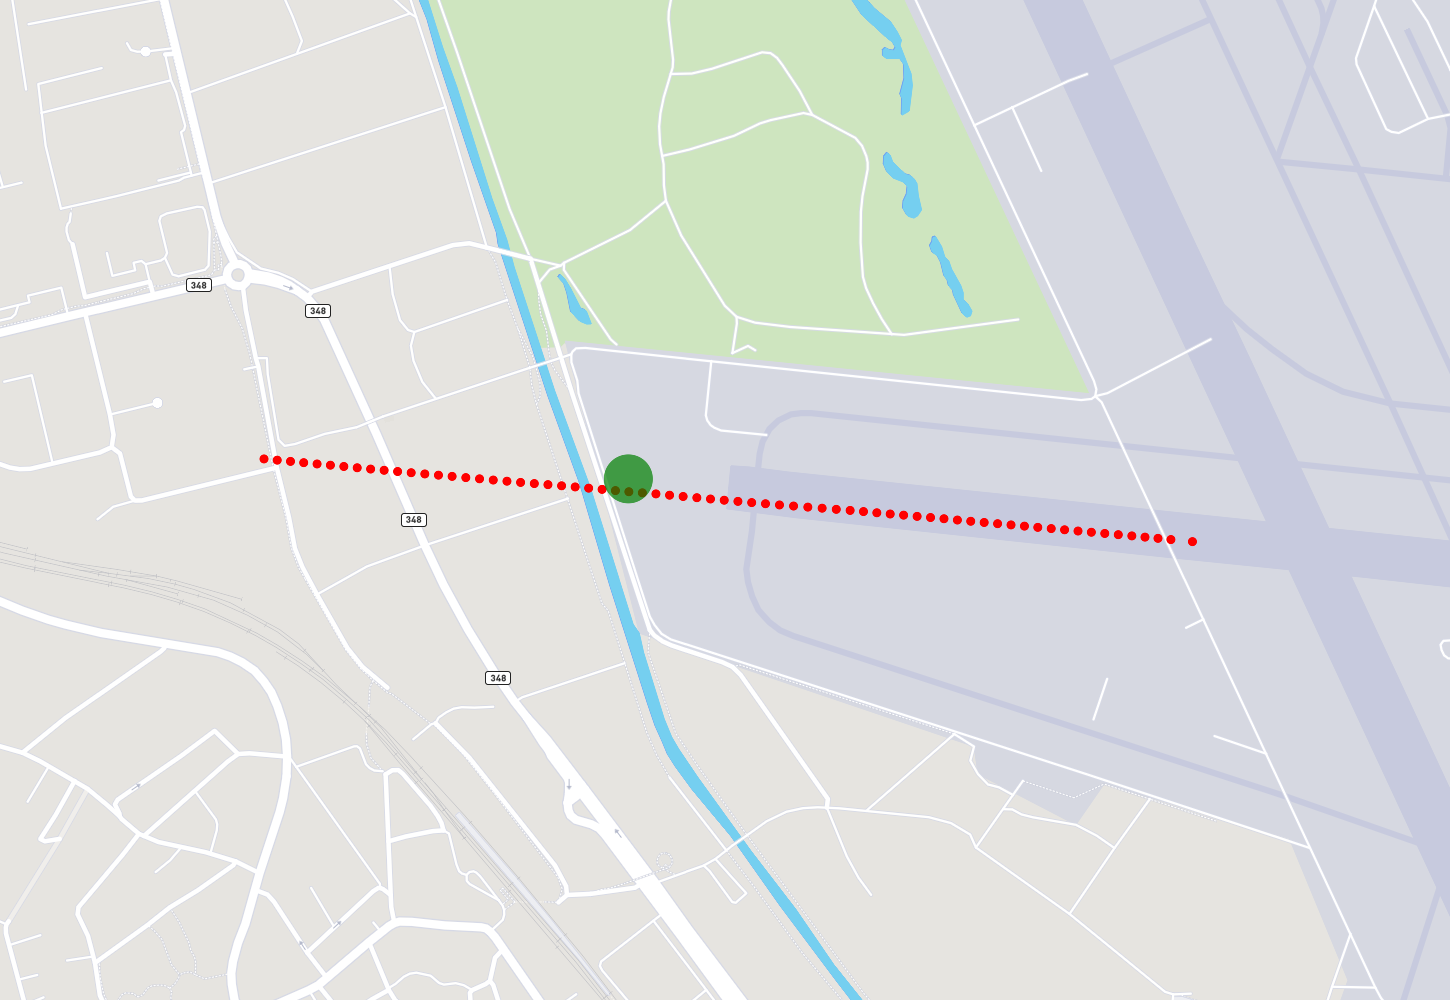
\includegraphics[width=0.5\textwidth]{../figures/manual/auralisation-paper/figure_trajectory}
  \caption{Overview of the airport, trajectory and the receiver. The receiver considered
(green dot) is situated slightly north of the trajectory, almost straight underneath the
trajectory.}
  \label{fig:figure_trajectory}
\end{figure}


\subsection{Backpropagation}
An automated procedure was developed to backpropagate from receiver to source in
time-domain. The procedure assumes there is only one propagation path,
the direct path, and that the aircraft can be considered a point source.
As shown in Figure \ref{fig:backpropagation_block_diagram}, the
backpropagation algorithm undoes atmospheric attenuation, the Doppler shift, and
geometrical spreading (magnitude) in that specific order, and using the methods as
described in the previous section.
% A recording is taken, and assuming there were no reflections, the atmospheric attenuation and spherical spreading were undone.
Because only the direct path was considered all parameters that were used in the
backpropagation were based on values corresponding to that path.

\begin{figure}[H]
  \centering
\begin{tikzpicture}[auto, node distance=1cm,>=latex']
\tikzset{
block/.style    = {draw, shape=rectangle, fill=white, minimum height=4em, minimum width=5em, text width=5em, align=center},
}
    % Main nodes
    \node [block]                       (immission)     {Immission\\Recording};
    \node [block, right=of immission]   (attenuation)   {Attenuation\\Filter};
    \node [block, right=of attenuation] (delay)         {Spreading\\Delay};
    \node [block, right=of delay]       (spreading)     {Spreading\\Gain};

    % Main edges
    \draw [->]  (immission)     --  (attenuation);
    \draw [->]  (attenuation)   --  (delay);
    \draw [->]  (delay)         --  (spreading);

\end{tikzpicture}
  \caption{Block diagram of the backpropagation model. These steps are applied sequentially to a recording in order to obtain a signal in time-domain that corresponds to the emission of the aircraft.}
  \label{fig:backpropagation_block_diagram}
\end{figure}

Application of the backpropagation algorithm results in a time-domain signal
that corresponds to the emission of the aircraft. The emission includes the
effect of convective amplification, i.e., the directivity effects due to source
motion.

The influence of the ground reflection is non-negligible. The backpropagation
model does not undo the ground reflection because it was not expected that this
would result in improved results due to the approximations that would have to be
made. For example, let us assume two clear propagation paths exist. The
immission consists of the contributions from each path. The propagation delays
of each contribution are different. The contributions are therefore
Doppler-shifted differently, and the contributions are generated at different
emission times. Minor differences in emission may exist also due to the
directivity. Furthermore, the reflection coefficient plays a large role and is
only roughly known.

In order to account for the extra contribution, a correction is applied. A soft
ground is still relatively hard and therefore a -3 dB correction was applied to
the power of the features obtained in the next section. Ideally, a microphone on
the ground was used, but the dataset that was available consisted of recordings
at a height of 4 meters.

Figure \ref{fig:recording} shows a spectrogram of a recording. Clearly visible
are the Doppler-shifted tones and the peaks due to atmospheric turbulence. The
most powerful tone corresponds to the blade passing frequency of the fan. The
other tones are Buzz-Saw tones.

Figure \ref{fig:backpropagated} shows a spectrogram of the recording after
backpropagation. The signal after backpropagation is shorter than the recording
due to lack of aircraft position information during the initial propagation
delay. The Doppler-shift has mostly been removed. Aside from small variations,
the tonal components remain constant in frequency over time. The variations are
caused by uncertainties in the measured position of the aircraft and thus the
estimated propagation delay. Artifacts like the mirror-effect and amplitude
modulations due to atmospheric turbulence remain.

\begin{figure}[H]
  \centering
  \includegraphics[]{../figures/generated/recording-to-auralisation/recording}
  \caption{
    Spectrogram of a recording of an A320. }
  \label{fig:recording}
\end{figure}

\begin{figure}[H]
  \centering
  \includegraphics[]{../figures/generated/recording-to-auralisation/reverted}
  \caption{Spectrogram of the recording shown in Figure \ref{fig:recording} after backpropagation to the source.}
  \label{fig:backpropagated}
\end{figure}

\subsection{Feature extraction}\label{sec:tool:emission:features}
Spectral modelling synthesis was chosen as emission synthesis strategy. With
spectral modelling synthesis a signal is generated as a superposition of tones
and bandpass-filtered noise.
% In order to synthesise the emission of the aircraft
% We're interested in entirely synthesizing the emission of the aircraft and chose to use
% spectral modelling synthesis, that is, a method where a signal is generated
% through a superposition of sines and noise.
Therefore, a method is needed to extract from the backpropagated recordings the
frequency, phase, and level of the tones, as well as the level of the noise as
function of frequency. This section presents a method that was developed for
extracting these features.

The situations considered are take-offs, and therefore the tonal components in
the spectra are not only the blade passing frequency of the fan and its
harmonics, but also \say{Buzz-Saw} tones. The common denominator of the
frequencies of these components is the frequency at which the engine shaft
rotates.

\subsubsection*{Motivation for method}
The events considered are short, typically less than 30 seconds, and their
spectra vary considerably over time due to directivity of the source. Thus, in
order to get a sufficiently good directivity resolution, a high temporal
resolution is needed, and that limits the possibility to average over time. The
frequency resolution, however, also matters. The emission may contain Buzz-Saw
harmonics with a fundamental frequency below 100 Hz. While that gives some
freedom for using a lower frequency resolution, first the actual tonal
components need to be detected and thus distinguished from the broadband noise.

While already corrected for in the backpropagation, the Doppler shift may make
it difficult connecting obtained frequency-components at one step to those
obtained the step later. Therefore, frequency-tracking algorithms were
considered \cite{Lampert2010}, notably Hidden Markov Models. Due to their
complexity such solutions were not pursued further.

Tone-detection in the frequency-domain is in its simplest form a matter of peak
detection for which a range of algorithms is known. However, a robust algorithm
is needed that can distinguish between the tonal components and broadband noise
peaks.

Initially, the complex cepstrum\footnote{The complex cepstrum is defined as
$c[n] = F^{-1}\left\{\log_{10}{\left( F \left\{x[n]\right\} \right)}\right\}$.}
was used to determine the fundamental frequency of the Buzz-Saw harmonics
(Paper \ref{paper:euronoise2015}). The method was reliable for determining the
fundamental frequency. Because all the tonal components considered are multiples
of this fundamental frequency, all their frequencies would then be known as
well. Unfortunately, the frequency-resolution, or more precisely the
quefrency-resolution, was not high enough to reliably predict the frequency of
the high-frequent components.

\subsubsection*{Tone-seeking algorithm}
Annex C of ISO 1996-2:2007 \cite{ISO1996-2_2007} describes an objective method
for assessing the audibility of tones in noise and a significant part of the
method describes a tone-seeking algorithm. The tone-seeking algorithm works in
frequency-domain on a narrowband power spectrum. An estimate of the narrowband
spectrum is obtained using Welch's method. The time signal is split in chunks, a
Hanning window is applied to each chunk, and a modified periodogram is determined for
each chunk. Finally, linear averaging over the chunks results in Welch's
estimate of the power spectral density.

In frequency-domain, the tone-seeking algorithm first determines noise pauses,
which are local maxima with a probability of a tone. Noise pauses span multiple
frequency lines, and their starts and ends can be found when the difference
between two adjacent lines is larger than $\Delta$ dB, where $\Delta$ is the
tone-seeking criterion. The next step is to assess whether tones exist in these
noise pauses. Each frequency bin or line is assigned a label indicating whether
it is part of a tone or whether it is masking noise.

The power of the lines that are part of a tone are integrated. A correction is
made for the masking noise contributions to those lines by estimating their
contribution from a regression through the lines marked as noise within a
portion of the critical band\footnote{A critical band is the bandwidth of a
filter created by the cochlea, the auditory part of the inner ear.} around the
centerfrequency of the tone. Furthermore, a 1.8 dB correction is applied as
correction for the Hanning window.

\subsubsection*{Extension and modifications}
The tone-seeking algorithm is capable of detecting many of the tonal components
but not all of them. Therefore, the algorithm is modified and extended (Paper \ref{paper:internoise2016}).
Because the tones of interest are all multiples of a
fundamental frequency, the goal is to determine this fundamental frequency
sufficiently accurate. The assumption was therefore made that all tones found by the
tone-seeking algorithm from the standard were harmonics and that the fundamental
frequency was within a specified range.
The fundamental frequency is then given
\begin{equation}
 f_{0} = \mathrm{gcd}\left(f_1, f_2, \dots, f_n \right)
\end{equation}
where $\mathrm{gcd}$ is the \emph{greatest common divisor}.
Implementations of the $\mathrm{gcd}$ operator attempt to find an exact solution.
Due to errors in the estimation of the frequency of the tones and because some tones are
not harmonics, an exact solution does not exist. Given an initial estimate of
the fundamental frequency, one could define an error as the sum of the squared
deviation between the target order of the harmonics and the actual estimated
order
\begin{equation}\label{eq:tool:features:error}
 e = \sum_{i=0}^{n} \left( \frac{f_i}{f_0} - \mathrm{round}\left(\frac{f_i}{f_0}\right) \right)^2
\end{equation}
An estimate of the fundamental frequency is obtained by minimising this error.

According to the standard an A-weighted signal should be used. Because the
frequencies of the tonal components are of interest, and not their audibilities,
an unweighted signal is considered instead. Because at the start and the end of
the signal the signal-to-noise is relatively low, the backpropagation algorithm
may cause unwanted amplification of the background noise. Therefore, the signal
was low-pass filtered with a \nth{4} order Butterworth low-pass filter with a
cut-off frequency at 10 kHz. Furthermore, in order to obtain an accurate
estimation an averaging-time of one minute is required, however, this could not
be done as explained. Instead, two-second windows without overlap were used, and
these windows were divided into 10 chunks in order to estimate a power spectrum
with a resolution of about 5 Hz. A two-second window proved to be a good balance
between temporal resolution and frequency resolution.

The tone-seeking algorithm is first ran with a tone-seeking criterion of 1 dB to
detect tonal components and obtain their centerfrequencies. A fundamental
frequency estimation is then done by minimising the error in equation
\eqref{eq:tool:features:error}. The next step is to determine the power of all
harmonics. That was done by explicitly setting noise pauses for each of the
harmonics, forcing the tone-seeking algorithm to determine tones.
The noise-pause bandwidth was set to a value that was a function of the fundamental
frequency $f_0$ in order to automatically scale. Because adjacent noise pauses
should not overlap the bandwidth should be smaller than $f_0$. The noise pause
bandwidth was set to $0.2 f_0$ as this value appeared to work well for
estimating the power of the \say{Buzz-Saw} harmonics. The level of the tones are
then estimated as described by the standard.

The broadband noise or \say{masking noise} was integrated in
\nicefrac{1}{6}-octaves and a Hanning-window correction of 1.8 dB was applied.
The -3dB bandwidth of the tones was recorded as well, although these values may
be inaccurate due to the 5 Hz frequency-resolution. The bandwidth of the tonal
components depends on various aspects, like frequency or phase modulations at
the source or during propagation, e.g. due to atmospheric turbulence. The direct
and reflected contribution are Doppler-shifted slightly differently and that
causes either double peaks or a single broader peak. But also averaging time and
window shape play a role.

% An earlier version of the algorithm did not use the $\mathrm{gcd}$ in
% combination with the optimisation algorithm but instead determined the
% fundamental frequency using the complex cepstrum (Paper ).
% While it was possible to reliably determine the fundamental frequency with the
% complex cepstrum, the value which was obtained was not sufficiently accurate
% for determining higher harmonics.

% In the method as described in Annex C of ISO 1996-2:2007 each spectral line is
% assigned a label, e.g. whether the line is part of a tone or noise. Tones
% typically have a bandwidth and can therefore, depending on the frequency
% resolution, be spread over multiple lines. In order to compute the level of a
% tone, the spectral lines corresponding to that tone need to be integrated.

% The center frequencies of the tonal components obtained with the enhanced method
% were fed back in the method of the standard to obtain labels for each spectral
% line and to compute the levels of the tones and the noise.

% The lines that were assigned noise were integrated into \nicefrac{1}{6} octaves and for each
% fractional octave its level was kept.

% For the feature extraction two seconds windows were used, without overlap.
% While a short window decreases frequency resolution and precision of the
% features, a short
% window was required in order to provide temporal resolution of the features.
%  A value for the phase could not be obtained because
% the signal was too noisy.

% For the development of an emission model it is expected that
% the uncertainties could be reduced through ensemble averaging. % TODO include this?

\subsection{Emission and immission synthesis}\label{sec:tool:synthesis:synthesis}
% As mentioned before the emission was synthesised using spectral modelling
% synthesis.
With the extracted features, which were obtained as function of time and at
several receiver positions, it is possible to develop an emission model that
takes into account directivity of the spectral components. Such emission model
would then output input for the SMS synthesiser, and the created emission signal
would be propagated to a receiver location.

An important question to ask is whether the described methodology of extracting
features, synthesising an emission signal and propagating it would result in
plausible auralisations. For example, it could be possible that the chosen
synthesis strategy and features cannot reproduce certain characteristics in the
sound. Therefore, the next chapter describes a comparison between auralisations
and recordings with the auralisations based on recordings.

For a specific event and receiver, the immission was backpropagated and features
were extracted. These features were used to re-synthesise the emission. The
emission signal was propagated to the receiver, and a direct path and a single
reflection were considered. The assumption was made that the emission is
identical for the emission angles corresponding to direct and reflected path.

The feature extraction method provided frequencies and levels of tonal
components as function of time. Variations in the frequencies as function of
time could be observed, but with a two second window that would result in only
few data points. Variations in frequency were therefore ignored and computed was an
average value for the fundamental and each of the harmonics.

As mentioned in the previous section, values for the phase of the tones could
not be obtained, and therefore values had to be chosen. Because the harmonics
are \say{Buzz-Saw} noise, a phase corresponding to a sawtooth signal was
initially assumed. Participants in a preliminary test found the simulations
sound metallic compared to the recordings (Paper \ref{paper:internoise2016}).
Therefore, the assumption was made that the initial phase relation between the
Buzz-Saw tones was entirely lost and could therefore be chosen randomly, in
which case the probability distribution would likely be uniform as otherwise a
certain initial phase would still be preferred.

Figure \ref{fig:synthesis} shows a spectrogram of the emission synthesis. The
level of the tonal components and the broadband noise varies over time. The
blade passing frequency is not clearly visible. The feature extraction algorithm
underestimated the levels of the blade passing frequency and its harmonics. As
explained in \ref{sec:tool:emission:features} tones were searched for in noise
pauses. These noise pauses were \say{created} after the fundamental frequency
was determined. The bandwidth of these noise pauses was relatively small because
they were tuned for the \say{Buzz-Saw} tones. An improvement would be to look in
a larger noise pause bandwidth or bandwidth for these tonal components, however,
that requires explicit knowledges of the amount of blades.

Figure \ref{fig:auralisation} shows a spectrogram
of the auralisation at the receiver. The Doppler-shifted tones and the
mirror-effect are clearly visible. The Doppler-shifted tones are not very
smooth. This is due to fluctuations in the measured aircraft position and a smoothing filter
could reduce impact of these uncertainties.

\newpage
% \afterpage{
\begin{figure}[H]
  \centering
  \includegraphics[]{../figures/generated/recording-to-auralisation/synthesis}
  \caption{Emission synthesis of the aircraft. Inputs to the emission synthesiser were obtained by applying the feature-extraction algorithm to the signal shown in Figure \ref{fig:backpropagated}.}
  \label{fig:synthesis}
\end{figure}


\begin{figure}[H]
  \centering
  \includegraphics[]{../figures/generated/recording-to-auralisation/auralisation}
  \caption{Auralisation of the event shown in Figure \ref{fig:recording} .
  }
  \label{fig:auralisation}
\end{figure}
% }
